\documentclass[12pt]{article}
\usepackage[utf8]{inputenc}
\usepackage{graphicx}
\usepackage[a4paper,width=150mm,top=25mm,bottom=25mm]{geometry}

\title{

\\
{COS 301 User Manual}
}



\author{Ctrl Alt Defeat}

\begin{document}

\begin{titlepage}
    \centering



    \vspace{2cm}
    \hrulefill\\
    \vspace{1cm}
    {\Huge\bfseries SRS Documentation v3.0}

    \vspace{1cm}

    {\Large Software Requirements Specification Document for\\Domain Pulse}\\
    \vspace{1cm}
    \hrulefill\\

    \vfill

    {\large Ctrl Alt Defeat}

    \vspace{1cm}

    {\large 2023/07/31}\\
    %    \vspace{1cm}
    %    \vspace{1cm}
    %    
\includegraphics[width=10cm]{../../Images/dpLogo.png}
    %    \vspace{1cm}\\
    %    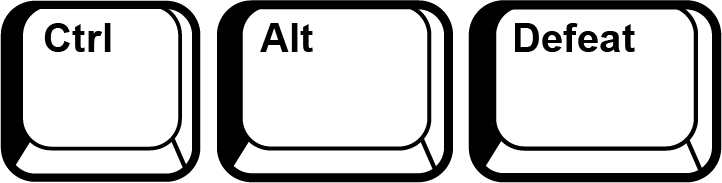
\includegraphics[width=6cm]{../../Images/cadLogo.png}

\end{titlepage}



\tableofcontents

\newpage



\section{Introduction}
\subsection{What is Domain Pulse?}
\begin{itemize}
    \item First we need to understand what Sentiment analysis is , Sentiment analysis is the process of computationally identifying and categorizing opinions expressed in a piece of text, especially in order to determine whether the writer's attitude towards a particular topic, product, etc. is positive, negative, or neutral. Now in this being said we introduce Domain Pulse.
    \item Domain pulse is the ultimate sentiment analysis platform. It gathers and analyses online opinions about any domain, be it a business, a person, or more. With stunning visuals and easy-to-understand statistics, Domain Pulse helps you understand the online presence and sentiment for any domain.
    \item Domain Pulse presents the results in a visually stunning and easy-to-understand
    format. Our wide range of visualisations bring statistics to life, which make it a breeze
    to grasp the online presence and sentiment for any domain. Take control of
    understanding public opinion like never before with Domain Pulse.
\end{itemize}
\subsection{Objectives of Domain Pulse}
\begin{itemize}
    \item The main objective of Domain Pulse is to provide a platform for users to analyse and gain valuable insight into the sentiment of any domain.
\end{itemize}
\newpage
\section{General access to the app}
\subsection{Logging into the app}
\begin{itemize}
    \item Simply add your email/username with which you registered with and your password and click on the blue 'login' button.
    \item Alternatively you can login with your Google account by clicking on the 'Sign in with Google' button.
    \item If you have forgotten your password, click on the 'Forgot Password?' link and follow the instructions.
    \item If you do not have an account, click on the 'Dont have an account?' link and register for an account using your chosen details.
\end{itemize}
\subsection{Registering for an account}
\begin{itemize}
    \item To register for an account the following information will be required:
    \begin{itemize}
        \item Username
        \item Email address
        \item Password
        \item Confirmation of password
    \end{itemize}
    \item Please enter the required information specified above in the relevant fields and click on the blue 'Register' button.
    \item If you already have an account , click on the 'Already have an account?' link and login with your registered details.
\end{itemize}



\end{document}
